\hypertarget{sec:results}{%
\chapter{Results}\label{sec:results}}

Here the resulting verification observations for the models \CGKAmod{\VersionOne}{}{} and \CGKAmod{\VersionTwo}{}{} are discussed.
As described above in Chapter\ \ref{sec:model-formalization}, the verification of the models are bounded, and hold only for the protocol prefixes up to \Tmax\ with at most \Nmax\ group members.
Verification was performed on each parameter combination for \CGKAmod{P}{T}{N} parameterized by \( \mathtt{P} \in \{\,\VersionOne,\, \VersionTwo\,\} \), \( T \in [\,4,\, \Tmax\ \,] \), and \( N \in [\,2,\, \Nmax\ \,] \).
The domain of each \CGKAmod{P}{T}{N} model parameter is listed in Table\ \ref{tab:model-param-domain}.
All observed verification results are tabulated in Appendix\ \ref{apx:Observations}.
At the time of submitting this thesis draft, a cursory glance will reveal that not all verification processes have completed.
These planned but incomplete observations are indicated by a \NA\ in table entries.


\hypertarget{performance-tuning}{%
\section{Performance Tuning}\label{performance-tuning}}

The performance and scaling of the verification efforts for \CGKAmod{}{}{} are contextualized.
Both time and memory constraints must be considered and a moderately comprehensive understanding of the verification tool Spin is required to correctly tune performance.
Spin supports many compile-time directives which allows for specifying the possible time-memory trade-off strategies which are desirable when verifying the specific model.
Not all compile time directives are compatible with all models.
Some directives require a proof by the user that certain conditions hold within the model for the directive's usage to be sound.
Furthermore, many directives' usage are are mutually exclusive with one or more other directives.
Still, with these restrictions in mind, the careful selection of compile-time directives is vital to successfully grappling with the enormity of memory usage resulting from the potentially exponential state-space explosion.


\hypertarget{sec:partial-order-reduction}{%
\subsection{Partial Order Reduction}\label{sec:partial-order-reduction}}

Partial-order reduction methods represent a well understood collection of state exploration techniques \autocite{godefroid1990using, godefroid1991using, godefroid1994partial} whose combined usage can greatly reduce the model checking search-space.
Such techniques are applicable for verifying local and termination of concurrent models.
Furthermore, these techniques are equally applicable for verifying LTL properties, even reducing the state-space when verifying liveness and safety properties within concurrent models.
The specific partial order reduction technique of ``simultaneous reachability'' analysis \autocite{van1997partial} enables the verification of non-executable transitions, absence of deadlock, and buffer overflows.
The extensive research and engineering effort put into the myriad of partial order reduction techniques have all been incorporated into verification strategies of SPIN, and are enabled by default,requiring manual ``opt-out'' compilation directives in order to disable them.
SPIN intelligently selects applicable partial order reduction techniques for the concurrency of the model, the LTL properties to be verified, and the topology of the state-space.
The verification work presented permitted the usage all the partial order reduction technique made available by SPIN.\@
No comparative verification(s) were made to observe the run-time difference between explicitly forbidding partial order reduction and permitting the ``enabled by default'' techniques available to SPIN.\@

The verification work refrained from from both disabling partial order reduction via the \texttt{NOREDUCE} directive as well as experimenting with potential performance gains or regressions introduced by the \texttt{NIBIS} directive.
Instead this work made use of a single partial order reduction directive:

\begin{itemize}
\item \texttt{XUSAFE}
\end{itemize}

The \texttt{XUSAFE} directive disables validity checks of the strictly synchronizing message passing queues.
The encoded model of TreeKEM does not utilize these queues, hence any check related to them would be superfluous.
Strict validity checks effects concurrency within the model, which in turn effects opportunities for partial order reduction.
No noticeable performance gains were observed by utilizing the \texttt{XUSAFE}, but its usage was retained regardless.


\hypertarget{sec:multi-core-tuning}{%
\subsection{Multi-core Tuning}\label{sec:multi-core-tuning}}

Since version 5.0, SPIN has supported performing model checking on multi-core machines \autocite{holzmann2007design}.
This support brings with it non-trivial engineering considerations, such as how to ensure partial order reduction remains sound across multiple independent processors, how to exchange search state results between processors, how to share or segregate memory, and how to minimize parallelism overhead.
There are two primary directives used my SPIN for approximating the optimal multi-core verification strategy at compile-time.
Both of these are used by this work while verifying TreeKEM.\@

\begin{itemize}
\item
  \texttt{MEMLIM=}\(X\)
\item
  \texttt{NCORE=}\(Y\)
\end{itemize}

The \texttt{MEMLIM} directive specifies the upper limit of memory usable by the model checker to be \(X\) Mebibytes for the duration its verification.
Specifying this has the important effect of preventing the verification process from thrashing by utilizing more virtual memory than real memory exists on the verification machine(s).
Moreover, the \texttt{NCORE} directive informs the model checker at compile-time the maximum number of usable processors is \(Y\), permitting the compiler to make informed approximations to minimize parallelism overhead and maximize multi-core throughput.
The verification work's utilization of both \texttt{MEMLIM} and \texttt{NCORE} directives when utilizing a multi-core computing cluster had notable impact on the overall ``states per second'' processing performance.


\hypertarget{sec:run-time-improvement}{%
\subsection{Run-time Improvement}\label{sec:run-time-improvement}}

Without any special direction SPIN includes a number of run-time checks and overhead structures to support functionality which may or may not actually be required for verification.
For each of these ``safety rails'' added to the verification by default, there exists a directive to remove the run-time feature.
The verification of TreeKEM does not require all run-time features and the following directives are used to remove the associated run-time increases.

\begin{itemize}
\item
  \texttt{NOBOUNDCHECK}
\item
  \texttt{NOFAIR}
\end{itemize}

The \texttt{NOBOUNDCHECK} directive removes run-time bounds checking when indexing arrays.
While enabled, the bound checking provides extremely useful debugging information.
Enabling bounds checking is useful while developing the model, but once confidence has been established that indexing errors do not exist in the model, such bounds checks are superfluous.
Additionally, the \texttt{NOBOUNDCHECK} performs run-time checks when synchronously accessing message queues.
The TreeKEM model does not use such message channels.
Consequently, the finalized model does not require bounds checking and the disabling directive is used during verification.

Similarly the \texttt{NOFAIR} removes the data structures and tracking subroutines required to reason about and verify fairness properties.
The verification of TreeKEM does not include any fairness properties.
Hence the \texttt{NOFAIR} directive is always enabled.


\hypertarget{reproducible-randomness}{%
\subsection{Reproducible Randomness}\label{reproducible-randomness}}

Like many problems with arbitrary alternation or stochastic search strategies, SPIN provides the opportunity for specifying seeds to exactly reproduce the results of random selection.
The benefits of reproducibility are difficult to understate.
Before the model is finalized, reproducibility is essential during the debugging process.
On the other hand, once the model is finalized, reproducibility is required for certainty during peer review.
Hence, directives for specify seed values are utilized throughout the verification work.

\begin{itemize}
\item
  \texttt{P\_RAND=}\(X\)
\item
  \texttt{T\_RAND=}\(Y\)
\end{itemize}

The first randomness directive, \texttt{P\_RAND}, is utilized to specify the random seed which determines process scheduling order for multi-process models.
The second, \texttt{T\_RAND} is also utilized, and corresponding the seed value dictates the transition exploration order when traversing the state-space.
Random seed values for \texttt{P\_RAND} and \texttt{T\_RAND} were set by manipulating the known numerical constants as defined below.
The transparency of the random seed value selection exists as a ``no tricks up my sleeve'' technique for specifying arbitrary seed values.

\begin{equation}
\begin{aligned}[t]
X = \texttt{1618033988} = & \bigg | \, \phi          \!\!\!\! & * \, 10^9 \, \bigg |\\
Y = \texttt{1155727349} = & \bigg | \, \frac{\pi}{e} \!\!\!\! & * \, 10^9 \, \bigg |\\
\end{aligned}
\end{equation}


\hypertarget{state-vector-encoding}{%
\subsection{State Vector Encoding}\label{state-vector-encoding}}

Each state within the model's state-space is encoded as a ``state-vector.''
The state vectors uniquely map to each state within the model.
Given that the main memory requirements of model checking lies in exhaustive state-space search, it is unsurprising that specifying the encoding of the state-vectors has a pronounced impact on memory usage.
There are many relevant directives used to influence the model checker's representation of state-vectors.
Note that all four directives listed below can be used in conjunction for compounding effects.

\begin{itemize}
\item \texttt{COLLAPSE}
\item \texttt{VECTORSZ=}\(X\)
\item \texttt{MA=}\(X\)
\item \texttt{SPACE}
\end{itemize}

The \texttt{VECTORSZ} directive is used to specify the number of byte \(X\) to allocate for each state-vector.
Specifying a number of bytes which is insufficient to represent the state vector will cause the compilation of the model to fail with an approximate suggestion of the correct number of bytes to specify.
The \texttt{VECTORSZ} directive is required when the state-vector length exceeds the SPIN default of \(1024\) bytes.
Likewise, the \texttt{COLLAPSE} directive applies compression the the state-vector representation.

A final two memory related directives are utilized conditionally during the verification of TreeKEM.\@
For large values of \(T\) and \(N\), the \texttt{MA} and \texttt{SPACE} directives are utilized in conjunction to increase the tractable values of \Tmax\ and \Nmax.
The conjunction of these two directives produces a very significant memory reduction, however the usage of \texttt{MA} causes an appreciable increase in verification run-time.
This time-memory trade-off is necessary to make verification of higher \Tmax\ and \Nmax\ values tractable, even on modern computing cluster hardware.

The \texttt{MA} directive is used to specify the maximum number of bytes \(X\) that a state vector can require.
Spin internally stores several sets of model states.
Using the information regarding the upper bound \(X\) for state-vector bytes, the \texttt{MA} directive enables a method of storing a set of states is a \Abrev{BDD} \autocite{holzmann1999minimized}.
To determine if the state is in the set, Spin treated the state vector as a bit-string and feeds it to the \Abrev{BDD}.
The state is contained within the set if the \Abrev{BDD} accepts the bit-string, and the state is not contained in the set if the \Abrev{BDD} rejects the bit-string.
Further steps are taken to reduce the \Abrev{BDD} into a minimal DFA representation of a 256-ary decision tree.
Insertion, deletion, and membership queries take linear time in the length of the state-vector.
The translation alone between DFA representation represents a stark time/memory trade-off, as linear time set membership is a stark difference between Spin's default hash-set storage method, resulting in reducing memory requirements while increasing verification run-time.

The \texttt{SPACE} directive instructs the compiler to encode the state transition graph as well as select search algorithms with the goal of reducing memory usage at the expense of verification time.
During verification of TreeKEM, it is always the case that the \texttt{SPACE} directive is utilized if and only if the \texttt{MA} is also utilized.
This conditional directive usage creates an ``optimization partition'' bifurcating verification runs into two sets of utilized directives.
An important consequence of this partitioning relates to comparative analysis of the verification run-time characteristics.
Such comparisons can only soundly be compared with other verification runs within the same set, utilizing the same directives.
In the tables presented below, the presence of a checkmark (\cmark) in the column labeled $\MinimizedDFA$ indicates that the associated parameterized model and results were run with this time/memory trade-off strategy enabled.
Table\ \ref{tab:state-vector-len} displays the state vector's byte length for each \CGKAmod{\VersionOne}{}{} parameterized model under verification.


\hypertarget{sec:verification-observations}{%
\section{Verification Observations}\label{sec:verification-observations}}

The model \CGKAmod{\VersionOne}{T}{N} was verified with as many possible parameters as time permitted.
The parameter space is listed in  Table \ref{tab:model-param-domain}.
Verification runs were performed on the American Museum of Natural History's Scientific Computing cluster.
The cluster job queue utilized, provides 1 TiB RAM and \(64\) AMD Opteron Processor 6380 core operating at 2500MHz.
Each verification run utilized 12 cores and up to 128 MiB of RAM.
Typically between five and six verification runs were performed concurrently by the cluster.
The observations of each \CGKAmod{\VersionOne}{T}{N} verification are depicted in Tables \ref{tab:V1-HLT}, \ref{tab:V1-FSU}, and \ref{tab:V1-PCS}.
Note that all run-times are ``wall clock'' time not ``CPU time.''

\hypertarget{sec:confidence-check}{%
\subsection{Confidence Check}\label{sec:confidence-check}}

The simplest of the three \Abrev{LTL} predicates defined in Section\ \ref{sec:LTL-security} is \LTLPredicate{HLT}.
The verification of \LTLPredicate{HLT} is successful if and only if in every possible execution of the model \CGKAmod{}{}{}, the program reaches the state \texttt{CGKA@start\_of\_epoch}.
While \LTLPredicate{HLT} is not truly a security property of \CGKAmod{}{}{}, it is used as a methodology confidence check.
Failure to verify \LTLPredicate{HLT} would cast serious doubt that the model verification methodology is being performed correctly on more complex \Abrev{LTL} predicates.
Verification results for \LTLPredicate{HLT} is displayed in Table\ \ref{tab:V1-HLT}.
All observations in Table\ \ref{tab:V1-HLT} report a successful verification of \LTLPredicate{HLT}.
From the observations obtained so far, one can conclude that the confidence check which has successfully verified \( \CGKAmod{}{}{} \models \LTLPredicate{HLT} \) does not introduce any doubt regarding the verification methodology.


\hypertarget{sec:post-compromise-security-results}{%
\subsection{Security Guarantees}\label{sec:post-compromise-security-results}}

The verification run observations for \LTLPredicate{FSU} are listed in Table\ \ref{tab:V1-FSU} and the verification run observations for \LTLPredicate{PCS} are listed in Table\ \ref{tab:V1-PCS}.
All observations in both Table\ \ref{tab:V1-FSU} and Table\ \ref{tab:V1-PCS} report a either successful verification of corresponding security guarantee or an ``out of memory'' error (\OutOfMemory).
These results are expected and consistent with prior literature regarding TreeKEM.
However, the confidence drawn from these verification results is limited by the size of the observation set.
Understanding the possibility of expanding the observation set is of great interest.


\hypertarget{sec:scalability-limits}{%
\section{Scalability Limits}\label{sec:scalability-limits}}

The state-vector lengths detailed in Table\ \ref{tab:state-vector-len} and columns observing verification performance within Appendix\ \ref{apx:Observations} provide an initial basis for interpreting the scalability of the \CGKAmod{P}{T}{N} model.
Considering the state-vector lengths alone, without considering the observed memory usage, a stark increase can be seen.
It is easy to notice that a progression from \( (\,T,\, N\,) \) to \( (\,T+1,\, N\,) \) is more significant in memory usage than a progression from \( (\,T,\, N\,) \) to \( (\,T,\, N+4\,) \).
The large jump in state-space and transition count between modeling successive epochs provides a secondary metric demonstrating this characteristic.
Hence the number of epoch the model is verified for drives the memory usage.
This intuitively makes sense, as each new epoch multiplicatively expands the diameter of the state-space.

While referencing Table\ \ref{tab:state-vector-len} and holding \(N = 8\) as a constant with \(T\) increasing, one can see that each incrementing of \(T\) required roughly an additional \(16\) bytes in state-vector length.
The increase in state-vector length by \(16\) bytes, or \(128\) bits, equates to potential increase of the states-space by \(2^{128}\)!
With absolute certainty, the verification problem increases exponentially.
Though much engineering effort has been taken to simplify the model encoding and adequately tune the performance via Spin directives, an exponential problem can only yield a small amount of tractability.

For each model, generally speaking, \(T = 7\) was the maximum value with resulted in a complete set of observations for all \(N \in [4, 8]\).
When \(T = 8\) and verification of both \LTLPredicate{FSU} and \LTLPredicate{PCS} properties was attempted with 128 MiB of RAM allotted, the verification prematurely terminated with an ``out of memory'' error (\OutOfMemory) for all \(N \in [4, 8]\)
It is immediately clear from the set of observations that both memory usage and verification run-time scales exponentially with increasing \(T\) and \(N\) parameters.
Additional computational resources and time will be required to extend the observation set to the desired range in Table\ \ref{tab:model-param-domain}.

The run-time observations for \(T \in [4, 7]\) were used as predictors to extrapolate an estimated for run-time for \(T \in [8, 12]\).
The projected run-times are depicted in Figure \ref{fig:runtime-projections} and tabulated in Table \ref{tab:predicted-run-times}.
Similarly, the projected CPU clock cycle requirements are tabulated in Table\ \ref{tab:predicted-cpu-ticks}.

\begin{figure}[ht!]
\centering
\caption[Run-time projections for \CGKAmod{\VersionOne}{T}{N}]{%
\label{fig:runtime-projections}%
Wall clock run-time projections for \CGKAmod{\VersionOne}{T}{N}\\%
$\forall\; N \in [4, 8]$ using $T \in [4, 7]$ as predictors for $T \in [8, 12]$.
}%
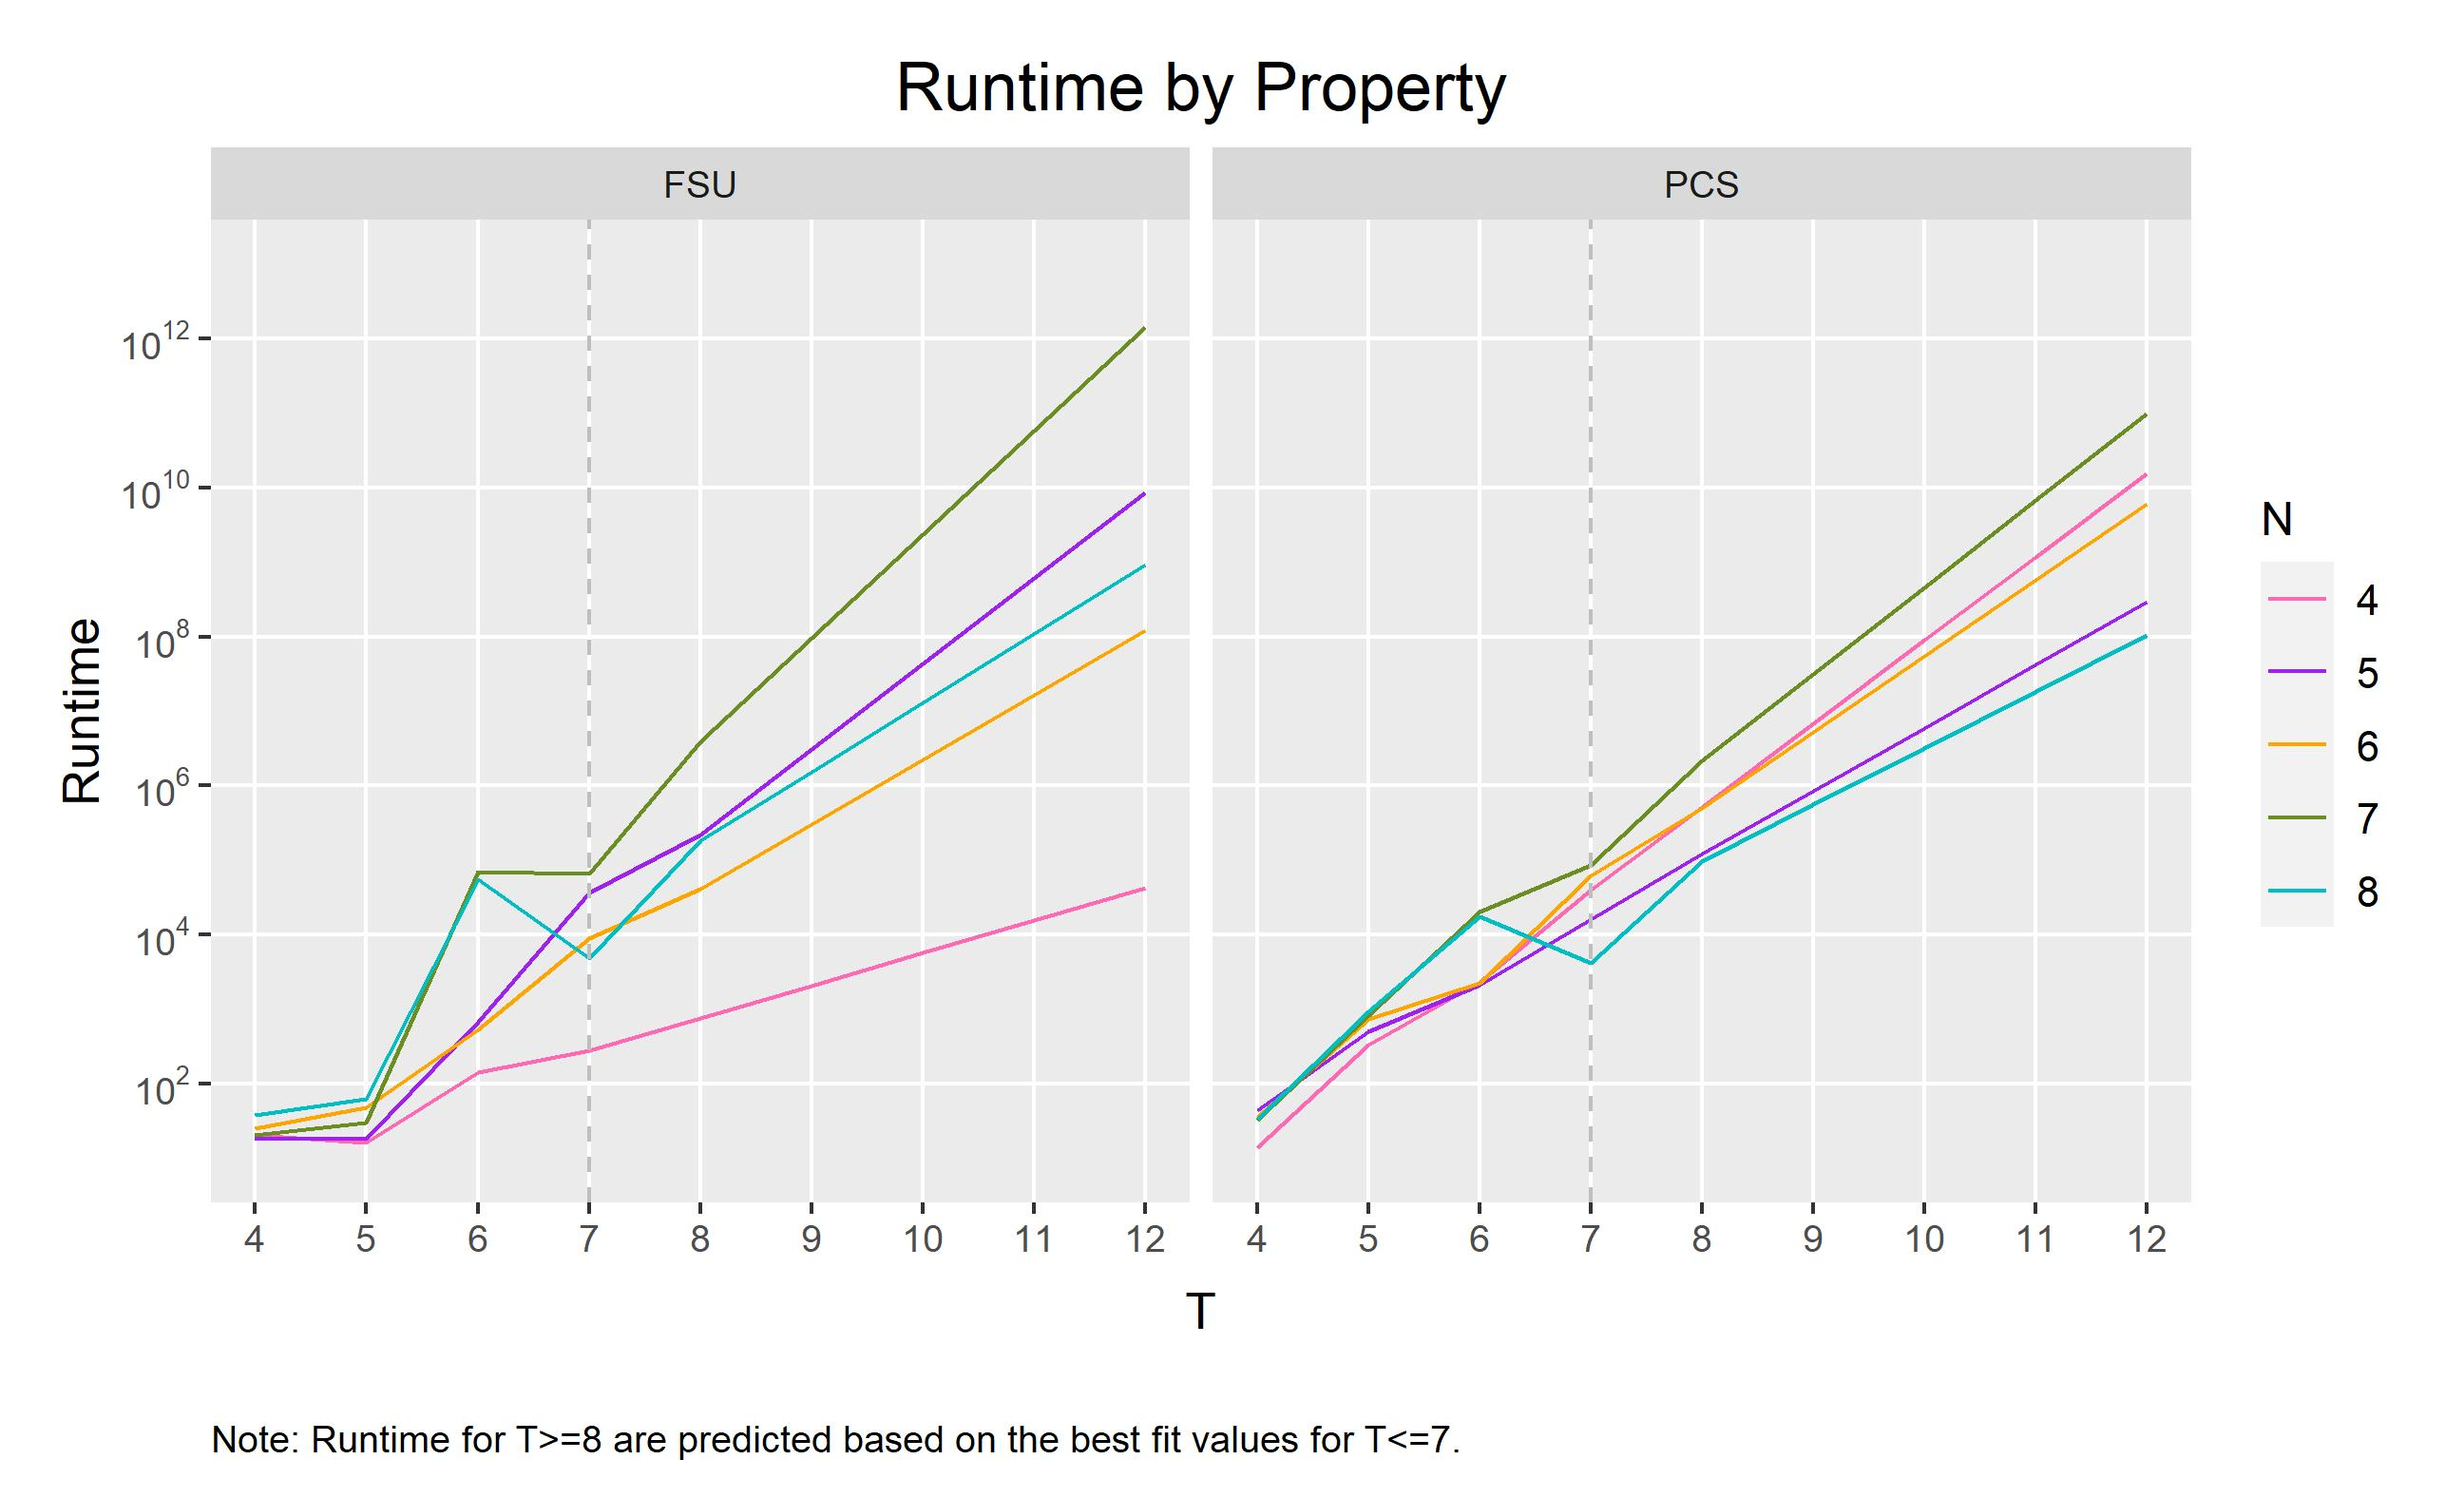
\includegraphics[width=\textwidth]{./figures/fsu-pcs-runtime-combined-preidcted.png}
\end{figure}

To estimate the required (wall clock) run-time, given the same computational hardware used for observations \(T \in [4, 7]\), to complete the observation set for the \CGKAmod{\VersionOne}{T}{N} parameter space \(\forall\; T \in [8, 12],\, N \in [4, 8],\, P \in \{ \LTLPredicate{FSU}, \LTLPredicate{PCS} \}\), one only needs to take the summation of the run-time estimates listed in Table \ref{tab:predicted-run-times}.
The summation amounts to an estimated \(1,639,073,974,176\) seconds of run-time.
Given the extremely optimistic case that six verifications can run concurrently and that the totaled verification run-time is perfectly divisible, one can divide the estimated seconds by six before concluding the estimated number of days required.
The divided summation yields an estimated \(273,178,995,696\) seconds of run-time.
Unfortunately, \(273,178,995,696\) seconds is equivalent to roughly \(8,657\) Gregorian years.
In order to complete the observation set by continuing with the same cluster hardware, further engineering improvements would be required with regard to performance tuning and model simplification.

Alternatively, if given sufficient additional cores and RAM matching the computational hardware used for observations \(T \in [4, 7]\) to run \emph{in parallel} the remaining observation set for the parameter space \(\forall T \in [8, 12], N \in [4, 8], P \in \{ \LTLPredicate{FSU}, \LTLPredicate{PCS} \}\), the (wall clock) runtime projection becomes much simpler to calculate.
The maximum predicted run-time estimate listed in Table \ref{tab:predicted-run-times} would indicate the total time required for all observations to be completed in parallel.
Given sufficient hardware for full parallelization of the remaining model parameters, completing the verification observation set would require only between 29 and 30 days.

In either case, more than 128 GiB of RAM would need to be allocated for each model verification with \(T \geq 8\).
From the observations for \(T \in [4, 7]\), it is difficult to confidently fit an exponential curve for projected memory usage of \(T \in [8, 12]\).
However, some preliminary scaling tests suggest that the requisite memory would exceed 512 GiB RAM for \(T = 12\).
Similarly, as shown in Table\ \ref{tab:predicted-cpu-ticks}, the projected CPU clock cycles required for \(T = 12\) would exceed \(62 \times 10^{15}\).
The conclusion of these hardware projections is that completion of the observation set within a reasonable time table will necessitate a large procurement of memory resources or further engineering efforts to reduce the memory footprint.
Specifically, parallel verification of 40 model parameterizations, each with 512 GiB to 1 TiB of RAM allocation and multiple CPU cores providing up to \(62 \times 10^{15}\) clock cycles.